\documentclass[12pt,a4paper,oneside]{book}

%% Package
\usepackage[latin1]{inputenc}
\usepackage{mathptmx, times}
\usepackage{amsmath, amsfonts, amssymb, amsthm}
\usepackage{thmtools,blindtext}
\declaretheoremstyle[%
spaceabove=1pt,%reduce or increase between theorem and proof
spacebelow=5pt,%reduce or increase
headfont=\normalfont\itshape,%
postheadspace=1em,%
qed=\qedsymbol%
]{mystyle} 
\declaretheorem[name={Bukti},style=mystyle,unnumbered,
]{pf}

\usepackage{graphicx, makeidx}
\usepackage{layout}
\usepackage{titlesec}
\usepackage{lipsum}
\usepackage[left=3.00cm, right=3.00cm, top=3.00cm, bottom=3.00cm]{geometry}
\usepackage{hyperref}
\usepackage{pgf,tikz}
\usepackage{mathrsfs}
\usetikzlibrary{arrows}
\usepackage{setspace}
\usepackage{hyperref}
\usepackage{cleveref}
\usepackage{enumitem}
\usepackage{fancyhdr}
\usepackage{multirow}
\usepackage{booktabs}
\usepackage{tabularx}
\usepackage{eucal}
\usepackage[Algorithm,ruled]{algorithm}
\usepackage{algpseudocode}
\usepackage{algorithmicx}
%\usepackage{algorithm,algorithmic}
\usepackage{rotating}
%\usepackage{sectsty}
\usepackage{booktabs}
\usepackage{amsthm}
\usepackage{titlesec}
\usepackage{multirow}
%\usepackage{filecontents}
\usepackage{titletoc}% http://ctan.org/pkg/titletoc
\usepackage[bahasa]{babel}
\usepackage[font=small]{caption}
%\usepackage[justification=centering]{caption}
\usepackage{subcaption}
\usepackage{float}
\usepackage{etoolbox}
\usepackage{ragged2e}
\usepackage{placeins}
\usepackage{breqn}

\usepackage{chngcntr}
\counterwithout{subsubsection}{subsection}

\captionsetup{format=hang}
\makeatletter %daftar pustaka
\renewcommand\@biblabel[1]{}
\makeatother

\titlecontents{chapter}% <section-type>
[0pt]% <left>
{\addvspace{1em}}% <above-code>
{\bfseries\chaptername\ \thecontentslabel\quad}% <numbered-entry-format>
{}% <numberless-entry-format>
{\bfseries\hfill\contentspage}% <filler-page-format>

\titleformat{\chapter}
{\filcenter\normalfont\large\bfseries}
{\chaptertitlename~\thechapter} {0.5em} {}
\renewcommand \thechapter{\Roman{chapter}}

\titlespacing{\chapter}{0pt}{0pt}{16pt}
\titlespacing{\section}{-5pt}{6pt}{-5pt}
\titlespacing{\subsection}{-5pt}{6pt}{-5pt}
\titlespacing{\subsubsection}{0pt}{6pt}{-5pt}

\setlength{\belowcaptionskip}{-10pt}

%\usepackage{blindtext, subfig}
%\usepackage{dblfloatfix}
%\captionsetup{compatibility=false}

\pagestyle{fancy}
\fancyhf{}

\onehalfspacing
\setlength{\parskip}{1em}
%\setlength{\parsep}{0em}
\setlength{\parindent}{0em}
%\setlist{nosep}

%\titlespacing*{\section}{0pt}{12pt plus 4pt minus 2pt}{0pt plus 2pt minus 2pt}
\titleformat{\section}{\normalfont\bfseries}{\sectiontitle~\thesection} {0.5em} {}
\titleformat{\subsection}{\normalfont\bfseries}{\sectiontitle~\thesubsection} {0.5em} {} {}

\include{hyphenation}
\frenchspacing

\theoremstyle{plain}
\newtheorem{lemma}{Lemma}[section]
\newtheorem{definisi}{Definisi}[section]
\newtheorem{akibat}{Akibat}[section]
\newtheorem{teorema}{Teorema}[section]
\newtheorem{bukti}{Bukti}[section]
\newtheorem{thm}{Teorema}[subsection]
\newtheorem{proposisi}{Proposisi}[section]
\newtheorem{observasi}{Observasi}[section]
\newtheorem{dugaan}{Dugaan}[section]
\newtheorem{masalah}{Masalah}[section]

\makeatletter
\newenvironment{breakablealgorithm}
{% \begin{breakablealgorithm}
	\begin{center}
		\refstepcounter{algorithm}% New algorithm
		\hrule height.1pt depth.1pt \kern-2pt% \@fs@pre for \@fs@ruled
		\renewcommand{\caption}[2][\relax]{% Make a new \caption
			{\raggedright\textbf{Algoritma~\thealgorithm} ##2}%
			\ifx\relax##1\relax % #1 is \relax
			\addcontentsline{loa}{algorithm}{\protect\numberline{\thealgorithm}##2}%
			\else % #1 is not \relax
			\addcontentsline{loa}{algorithm}{\protect\numberline{\thealgorithm}##1}%
			\fi
			\kern2pt\hrule\kern2pt
		}
	}{% \end{breakablealgorithm}
		\kern2pt\hrule\relax% \@fs@post for \@fs@ruled
	\end{center}
}
\makeatother

\newcommand{\overbar}[1]{\mkern 1.5mu\overline{\mkern-1.5mu#1\mkern-1.5mu}\mkern 1.5mu}


%% Title

\newcommand{\listexamplename}{DAFTAR LAMPIRAN}
%\newlistof{example}{exp}{\listexamplename}
\newcommand{\lampiran}[1]{%
	\refstepcounter{example}
	\par\noindent\textbf{LAMPIRAN  \theexample\quad #1}
	\addcontentsline{exp}{example}
	{{\theexample} #1}\par}

\pagenumbering{roman}
\makeindex

\author{Nama Mahasiswa}
\title{Judul Skripsi Anda}
\tolerance=1
\emergencystretch=\maxdimen
\hyphenpenalty=1000
\hbadness=1000

\begin{document}
	\onehalfspacing
	%\thispagestyle{empty}
	\frontmatter
% Cover
	\begin{titlepage}
\begin{center}

\includegraphics[height=2.5cm, width=2.1cm]{LogoITERA.png}\\[5ex]
\textbf{\fontsize{14pt}{0}\selectfont EVALUASI PERFORMA HADOOP DAN SPARK PADA CLOUD IAAS DENGAN MENGGUNAKAN HIBENCH BENCHMARKING DALAM KONFIGURASI PSEUDO DISTRIBUTED}\\
\vspace{3cm}

\textbf{\fontsize{14pt}{0}\selectfont  PROPOSAL PENELITIAN}\\[18ex]
\textbf{\fontsize{12pt}{0}\selectfont{Dimas Wahyu Saputro}}\\ 
\textbf{\fontsize{12pt}{0}\selectfont{120450081}}\\[20ex]
\textbf{\fontsize{12pt}{0}\selectfont PROGRAM STUDI SAINS DATA}\\
\textbf{\fontsize{12pt}{0}\selectfont JURUSAN SAINS}\\
\textbf{\fontsize{12pt}{0}\selectfont INSTITUT TEKNOLOGI SUMATERA}\\
\textbf{\fontsize{12pt}{0}\selectfont LAMPUNG SELATAN}\\
\textbf{\fontsize{12pt}{0}\selectfont 2024}\\
\vspace{3cm}
\end{center}
\end{titlepage}
	\begin{titlepage}
\begin{center}

\includegraphics[height=2.5cm, width=2.1cm]{LogoITERA.png}\\[5ex]
\textbf{\fontsize{14pt}{0}\selectfont PERBANDINGAN KINERJA ANTARA HADOOP DAN SPARK MENGGUNAKAN TOLOK UKUR HIBENCH}\\
\vspace{3cm}

\textbf{\fontsize{14pt}{0}\selectfont  TUGAS AKHIR}\\
\textbf{\fontsize{12pt}{0}\selectfont  Diajukan sebagai syarat untuk memperoleh gelar sarjana}\\[18ex]
\textbf{\fontsize{12pt}{0}\selectfont{Dimas Wahyu Saputro}}\\ 
\textbf{\fontsize{12pt}{0}\selectfont{120450081}}\\[20ex]
\textbf{\fontsize{12pt}{0}\selectfont PROGRAM STUDI SAINS DATA}\\
\textbf{\fontsize{12pt}{0}\selectfont JURUSAN SAINS}\\
\textbf{\fontsize{12pt}{0}\selectfont INSTITUT TEKNOLOGI SUMATERA}\\
\textbf{\fontsize{12pt}{0}\selectfont LAMPUNG SELATAN}\\
\textbf{\fontsize{12pt}{0}\selectfont 2024}\\
\vspace{3cm}
\end{center}
\end{titlepage}

	%\cleardoublepage
\centerline{\large\bfseries LEMBAR PENGESAHAN}
\phantomsection
\addcontentsline{toc}{chapter}{LEMBAR PENGESAHAN}
\vspace*{40pt}

Tugas Akhir dengan judul "Judul Skripsi Anda" adalah benar dibuat oleh saya sendiri dan belum pernah dibuat dan diserahkan sebelumnya, baik sebagian ataupun seluruhnya, baik oleh saya ataupun orang lain, baik di Institut Teknologi Sumatera maupun di institusi pendidikan lainnya.

\begin{table}[htbp]
	\begin{tabular}{p{9.8cm}p{4cm}}
		& \multirow{3}{*}{{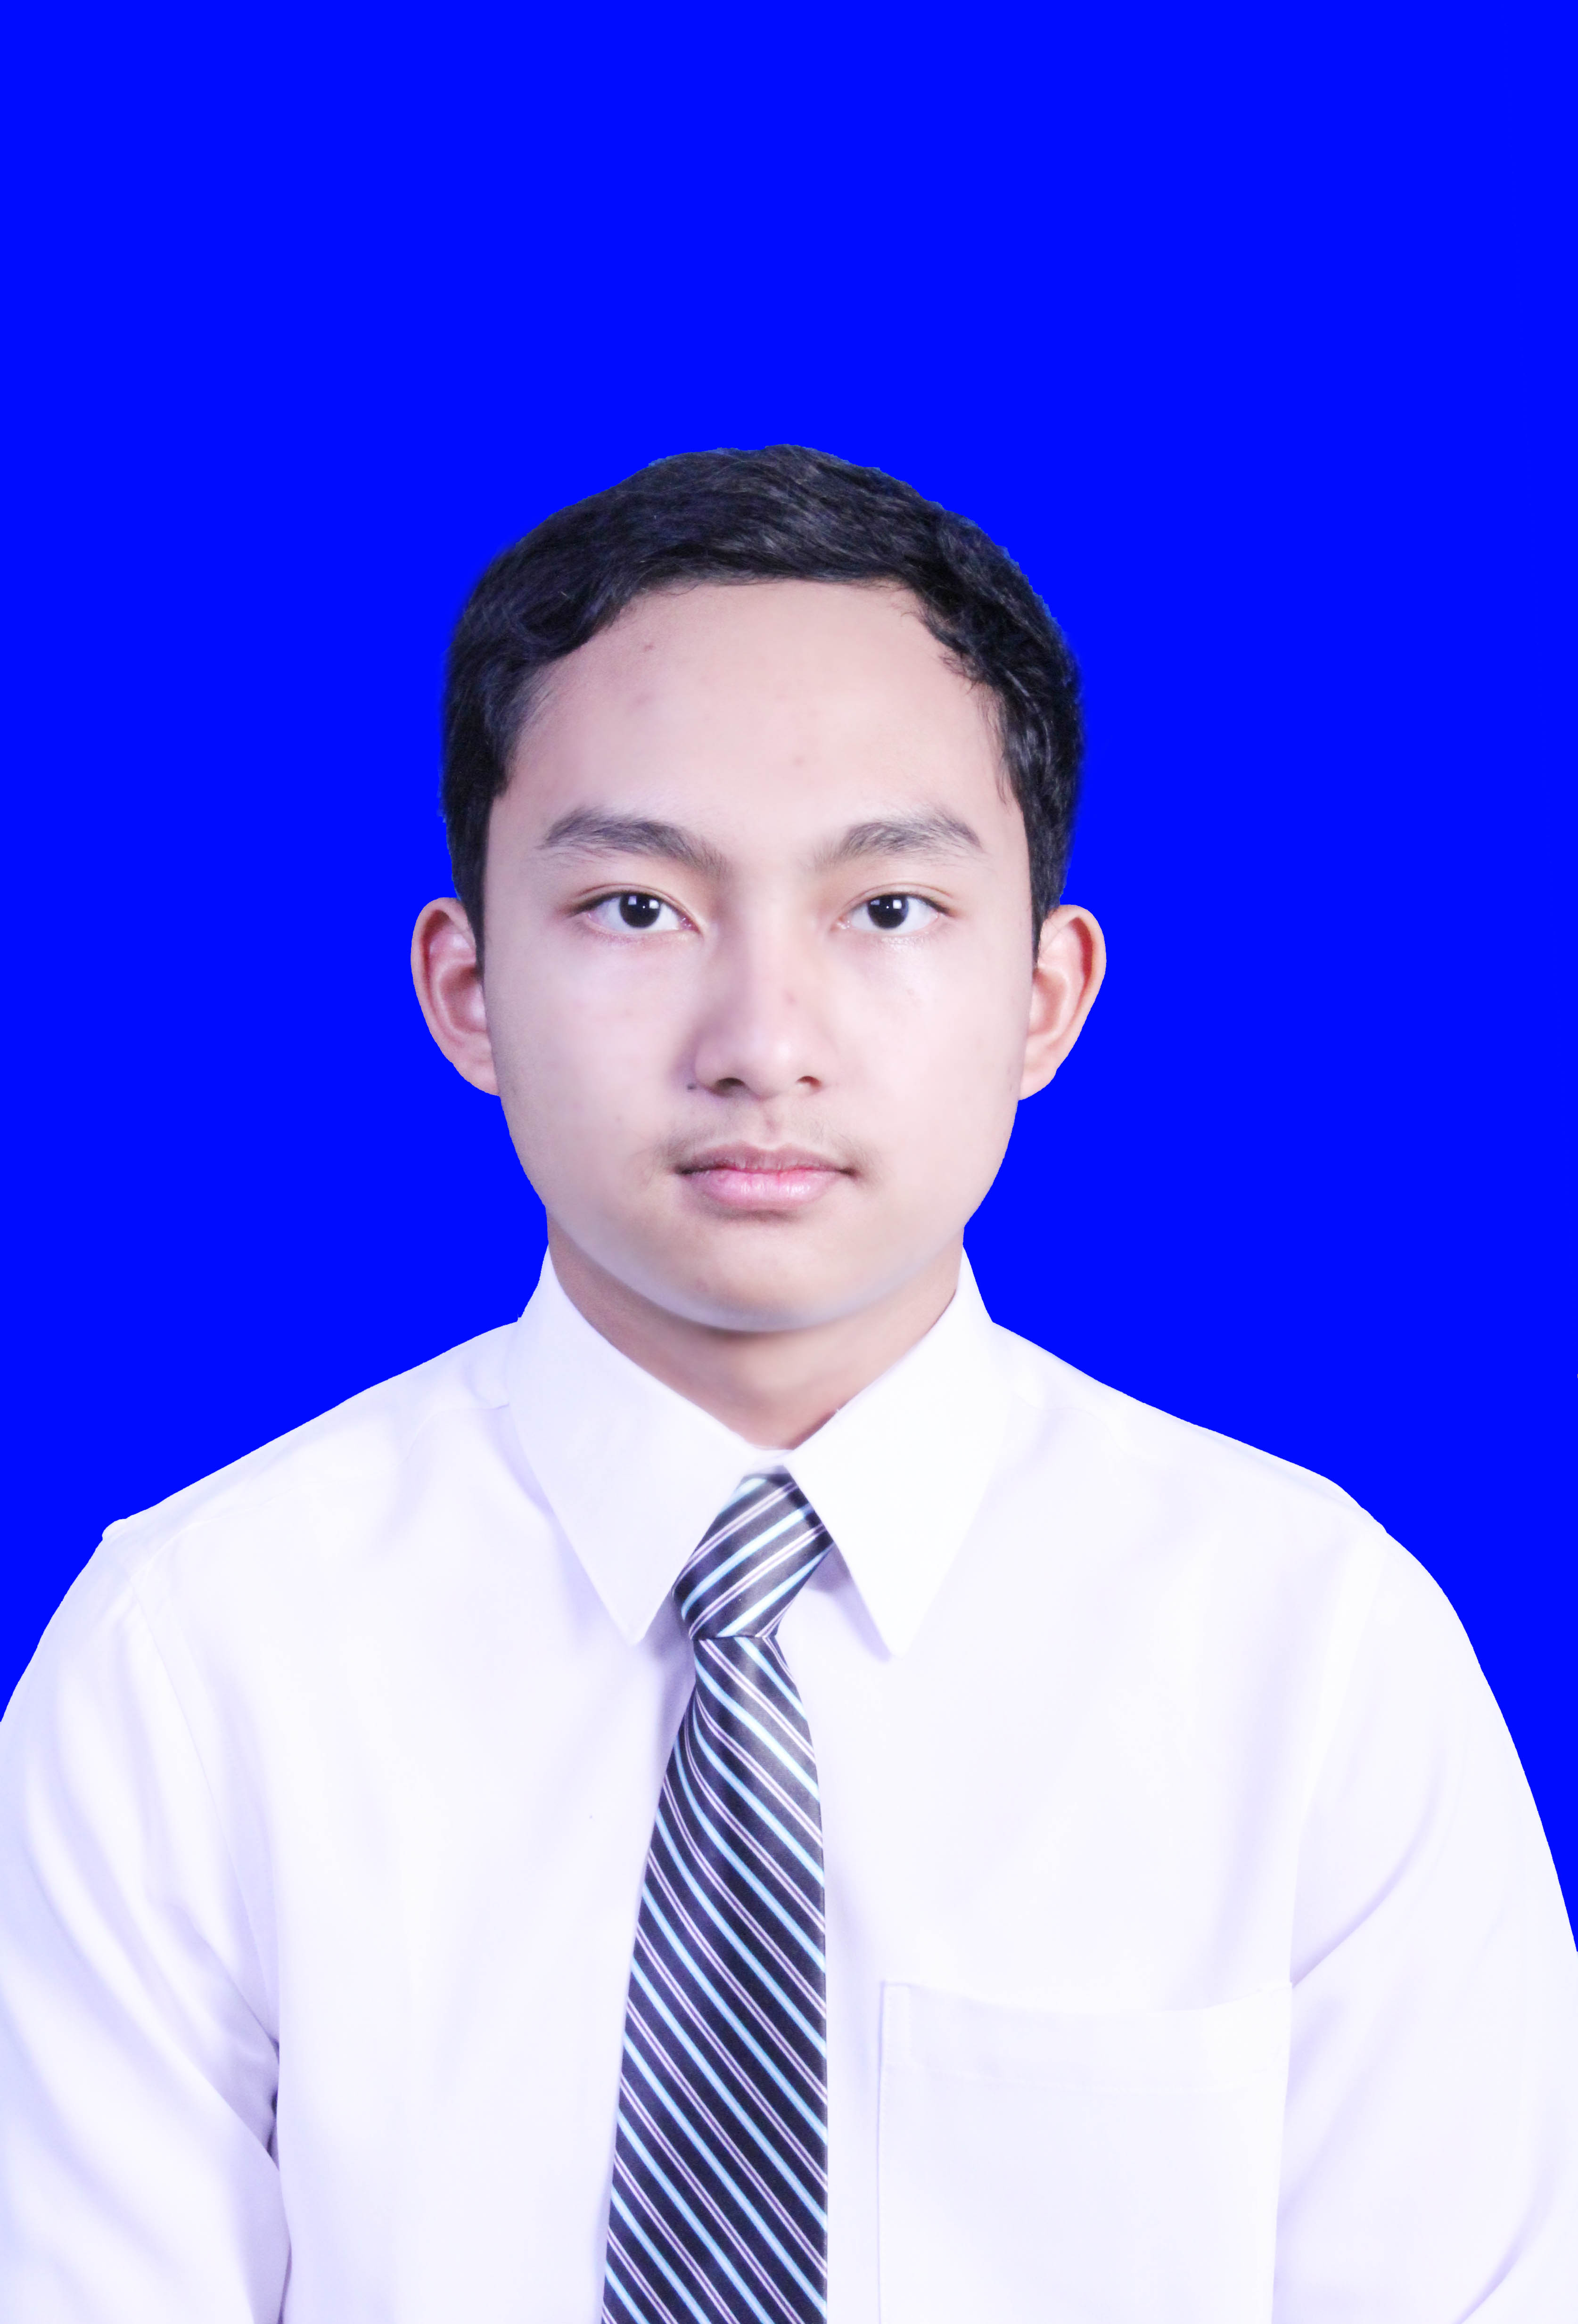
\includegraphics[width=3cm,height=4.5cm]{pasfoto.jpg}}} \\
		{Lampung Selatan, xx xxxx 20xx} & \\
		Penulis, & \\[8ex]
		Dimas Wahyu Saputro   & \\
		{NIM 120450081} & \\[9ex]
	\end{tabular}
\end{table}

\begin{center}
	\begin{tabularx}{\textwidth}{c@{}lXc@{}}%{ccc}
		Pembimbing I & & & Pembimbing II \\ [9ex]
		Nama Pembimbing 1 beserta gelar & & & Nama Pembimbing 2 beserta gelar \\ 
		NIP. xxxxxxxxxx & & & NIP xxxxxxxxxx
	\end{tabularx}
\end{center}

\begin{center}			
	{Disahkan oleh,} 	\\
	{Koordinator Program Studi Sains Data}\\
	{Jurusan Sains} \\
	Institut Teknologi Sumatera\\[9ex]	
	{Nama Koorprodi beserta gelar}\\
	{NIP xxxxxxxxxx}	
\end{center}





	\cleardoublepage
\centerline{\large\bfseries HALAMAN PERNYATAAN ORISINALITAS}
\phantomsection
\addcontentsline{toc}{chapter}{HALAMAN PERNYATAAN ORISINALITAS}
\vspace*{40pt}
\begin{spacing}{1}
\begin{center}\bf
	Skripsi ini adalah karya saya sendiri, dan semua sumber baik yang dikutip maupun dirujuk telah saya nyatakan benar.
	\vspace*{120pt}
	\begin{spacing}{1.5}
		\begin{tabular}{lcl}
				Nama &:& Nama Anda\\
				NIM &:& 1xx45xxxx\\
				Tanda Tangan &:&\\
				Tanggal &:& xx xxxx 20xx (Tanggal disetujui)
		\end{tabular}
	\end{spacing}
\end{center}
\end{spacing}

	\cleardoublepage
\centerline{\large\bfseries HALAMAN PERSETUJUAN PUBLIKASI}
\vspace*{1ex}
\centerline{\large\bfseries TUGAS AKHIR UNTUK KEPENTINGAN AKADEMIS}
\phantomsection
\addcontentsline{toc}{chapter}{HALAMAN PERSETUJUAN PUBLIKASI}
\vspace*{40pt}
Sebagai civitas akademik Institut Teknologi Sumatera, saya yang bertanda tangan di bawah ini:
\begin{spacing}{1.5}
	\begin{tabular}{lcl}
		Nama 			&:& Dimas Wahyu Saputro \\
		NIM 			&:& 120450081  \\
		Program Studi 	&:& Sains Data  \\
		Jurusan 		&:& Sains \\
		Jenis Karya 	&:& Laporan Tugas Akhir
	\end{tabular}
\end{spacing}
demi pengembangan ilmu pengetahuan, menyetujui untuk memberikan kepada Institut Teknologi Sumatera \textbf{Hak Bebas Royalti Nonekslusif \textit{(Non-exclusive Royalty Free Right)}} atas karya ilmiah saya yang berjudul:
\begin{center} \textbf{Judul Skripsi Anda}\end{center}
beserta perangkat yang ada (jika diperlukan). Dengan Hak Bebas Royalti Noneksklusif ini Institut Teknologi Sumatera berhak menyimpan, mengalihmedia/formatkan, mengelola dalam bentuk pangkalan data (database), merawat, dan memublikasikan tugas akhir saya selama tetap mencantumkan nama saya sebagai penulis/pencipta dan sebagai pemilik Hak Cipta.\\
Demikian pernyataan ini saya buat dengan sebenarnya.
\begin{center}
\begin{tabular}{rcl}
	Dibuat di 		&:&~Lampung Selatan\\
	Pada tanggal 	&:&~xx xxxx 20xx \\
\end{tabular}
\\[2ex]
Yang menyatakan,\\[10ex]
Dimas Wahyu Saputro
\end{center}

	
%\chapter{\textbf{ABSTRAK}}
%\begin{center}
%\textbf{{\LARGE{\textsc{MODEL PREDIKSI INAR(1) \\UNTUK STATUS KESEHATAN}}}}
%\end{center}
%\vspace{.8cm}
%\begin{center}
\addcontentsline{toc}{chapter}{ABSTRAK}
%\end{center}
\begin{center}
\textbf{\fontsize{12pt}{0}\selectfont{Judul Skripsi Anda}} \\
\vspace{14pt}
\textbf{\fontsize{12pt}{0}\selectfont{Nama Mahasiswa (1xx45xxxx)}}\\
\textbf{\fontsize{12pt}{0}\selectfont{Nama Pembimbing 1 beserta gelar}}\\
\textbf{\fontsize{12pt}{0}\selectfont{Nama Pembimbing 2 beserta gelar}}\\
\vspace{36pt}
\textbf{\fontsize{12pt}{0}\selectfont{ABSTRAK}}
\end{center}
\vspace{20pt}
\singlespacing
Abstrak yang dimaksudkan adalah ringkasan atau intisari, maksimum 200 kata atau satu halaman. Abstrak merupakan ikhtisar suatu tugas akhir yang memuat permasalahan, tujuan, metode penelitian, hasil, dan kesimpulan. Abstrak dibuat untuk memudahkan pembaca mengerti secara cepat isi tugas akhir untuk memutuskan apakah perlu membaca lebih lanjut atau tidak. Abstrak tidak memuat gambar maupun tabel, ditulis dengan huruf Times New Roman, 12 pt, satu spasi. Abstrak ditulis dalam bahasa Indonesia dan bahasa Inggris, masing-masing dimulai pada halaman baru. Abstrak hendaknya memuat satu kalimat yang menjelaskan latar belakang masalah, satu kalimat yang menjelaskan tujuan dan satu kalimat yang menjelaskan manfaat, satu kalimat yang menjelaskan lingkup dan satu kalimat yang menjelaskan batasan masalah, satu kalimat yang menjelaskan metodologi, percobaan maupun satu kalimat yang menjelaskan interpretasi data sertasatu kalimat yang menjelaskan hasil-hasil penelitian yang diperoleh. Di bawah abstrak, setelah satu baris kosong, tuliskan "Kata kunci:" diikuti lima kata kunci yang sesuai.


\singlespacing
\noindent 
\vspace{1ex}
\noindent
\begin{tabularx}{\textwidth}{@{}lX@{}}
    {\textbf{Kata kunci:}} & {Kata Kunci 1, Kata Kunci 2, Maksimal 5 Kata Kunci}
\end{tabularx}

	
%\chapter{\textbf{ABSTRAK}}
%\begin{center}
%\textbf{{\LARGE{\textsc{MODEL PREDIKSI INAR(1) \\UNTUK STATUS KESEHATAN}}}}
%\end{center}
%\vspace{.8cm}
%\begin{center}
\addcontentsline{toc}{chapter}{ABSTRAK}
%\end{center}
\begin{center}
\textbf{\fontsize{12pt}{0}\selectfont{Judul Skripsi Anda}} \\
\vspace{14pt}
\textbf{\fontsize{12pt}{0}\selectfont{Nama Mahasiswa (1xx45xxxx)}}\\
\textbf{\fontsize{12pt}{0}\selectfont{Nama Pembimbing 1 beserta gelar}}\\
\textbf{\fontsize{12pt}{0}\selectfont{Nama Pembimbing 2 beserta gelar}}\\
\vspace{36pt}
\textbf{\fontsize{12pt}{0}\selectfont{ABSTRAK}}
\end{center}
\vspace{20pt}
\singlespacing
Abstrak yang dimaksudkan adalah ringkasan atau intisari, maksimum 200 kata atau satu halaman. Abstrak merupakan ikhtisar suatu tugas akhir yang memuat permasalahan, tujuan, metode penelitian, hasil, dan kesimpulan. Abstrak dibuat untuk memudahkan pembaca mengerti secara cepat isi tugas akhir untuk memutuskan apakah perlu membaca lebih lanjut atau tidak. Abstrak tidak memuat gambar maupun tabel, ditulis dengan huruf Times New Roman, 12 pt, satu spasi. Abstrak ditulis dalam bahasa Indonesia dan bahasa Inggris, masing-masing dimulai pada halaman baru. Abstrak hendaknya memuat satu kalimat yang menjelaskan latar belakang masalah, satu kalimat yang menjelaskan tujuan dan satu kalimat yang menjelaskan manfaat, satu kalimat yang menjelaskan lingkup dan satu kalimat yang menjelaskan batasan masalah, satu kalimat yang menjelaskan metodologi, percobaan maupun satu kalimat yang menjelaskan interpretasi data sertasatu kalimat yang menjelaskan hasil-hasil penelitian yang diperoleh. Di bawah abstrak, setelah satu baris kosong, tuliskan "Kata kunci:" diikuti lima kata kunci yang sesuai.


\singlespacing
\noindent 
\vspace{1ex}
\noindent
\begin{tabularx}{\textwidth}{@{}lX@{}}
    {\textbf{Kata kunci:}} & {Kata Kunci 1, Kata Kunci 2, Maksimal 5 Kata Kunci}
\end{tabularx}

	\cleardoublepage
\centerline{\large\bfseries MOTTO}
\phantomsection
\addcontentsline{toc}{chapter}{MOTTO}
\vspace*{40pt}
%\begin{titlepage}
%\begin{center}
%\textbf{\fontsize{12pt}{0}\selectfont MOTTO}\\
%\vspace{3cm}

Penulisan motto bersifat optional/pilihan, tidak ada aturan dalam penulisannya
%\end{center}
%\end{titlepage}

	\cleardoublepage
\centerline{\large\bfseries PERSEMBAHAN}
\phantomsection
\addcontentsline{toc}{chapter}{PERSEMBAHAN}
\vspace*{40pt}
%\begin{titlepage}
%\begin{center}
%\textbf{\fontsize{12pt}{0}\selectfont HALAMAN PERSEMBAHAN}\\
%\vspace{3cm}

Penulisan halaman persembahan bersifat optional/pilihan, tidak ada aturan dalam penulisannya
%\end{center}
%\end{titlepage}

	\cleardoublepage
\centerline{\large\bfseries KATA PENGANTAR}
\phantomsection
\addcontentsline{toc}{chapter}{KATA PENGANTAR}
\vspace*{40pt}

Tuliskan maksud penulisan laporan, misal "Laporan penelitian ini dimaksud kan untuk memenuhi salah ".........Pada halaman ini mahasiswa berkesempatan untuk menyatakan terima kasih secara tertulis kepada pembimbing dan pihak lain yang telah memberi bimbingan, nasihat, saran dan kritik, kepada mereka yang telah membantu melakukan penelitian, kepada perorangan atau lembaga yang telah memberi bantuan keuangan, materi dan/atau sarana.

Cara menulis kata pengantar beraneka ragam, tetapi hendaknya menggunakan kalimat yang baku. Ucapan terima kasih agar dibuat tidak berlebihan dan dibatasi pada pihak yang terkait secara ilmiah (berhubungan dengan subjek/materi penelitian). Kata pengantar ditulis dalam satu halaman, huruf Times New Roman 12 pt, 1½ spasi, dengan marjin sesuai dengan marjin bagian tengah laporan.	

	\thispagestyle{myheadings}
	\renewcommand{\contentsname}{DAFTAR ISI}
	\pagestyle{fancy}
	%\pretocmd{\chapter}{\addtocontents{toc}{\protect\addvspace{5\p@}}}{}{}
	%\pretocmd{\section}{\addtocontents{toc}{\protect\addvspace{5\p@}}}{}{}
	%\singlespacing
	\newpage
	\addcontentsline{toc}{chapter}{\textbf{DAFTAR ISI}}
	\tableofcontents
	%\singlespacing
	\fancyhead[L]{\textsl{Daftar Isi}}
	\fancyhead[R]{}
	\fancyfoot[C]{\thepage}
	
	\parindent 0cm
	\makeatletter
	\renewcommand*\l@figure{\@dottedtocline{1}{1em}{3.2em}}
	\makeatother
	\renewcommand{\listfigurename}{DAFTAR GAMBAR}
	\listoffigures
	\addcontentsline{toc}{chapter}{\textbf{DAFTAR GAMBAR}}
	\pagestyle{fancy}
	\fancyhead[L]{\textsl{Daftar Gambar}}
	\fancyhead[R]{}
	\fancyfoot[C]{\thepage}
	
	\renewcommand{\listtablename}{DAFTAR TABEL}
	\makeatletter
	\renewcommand*\l@table{\@dottedtocline{1}{1em}{3.2em}}
	\makeatother
	\listoftables
	\addcontentsline{toc}{chapter}{\textbf{DAFTAR TABEL}}
	\pagestyle{fancy}
	\fancyhead[L]{\textsl{Daftar Tabel}}
	\fancyhead[R]{}
	\fancyfoot[C]{\thepage}
	
	\renewcommand{\listofalgorithms}{ 
		\begingroup 
		\listof{algorithm}{DAFTAR ALGORITMA} 
		\endgroup 
	}
	\makeatletter
	\renewcommand*\l@table{\@dottedtocline{1}{1em}{3.2em}}
	\makeatother
	\listofalgorithms
	\addcontentsline{toc}{chapter}{\textbf{DAFTAR ALGORITMA}}
	\pagestyle{fancy}
	\fancyhead[L]{\textsl{Daftar Algoritma}}
	\fancyhead[R]{}
	\fancyfoot[C]{\thepage}
	
%	\include{DaftarSDL}
	% BAB 1, BAB 2, BAB 3.
	\mainmatter
	\thispagestyle{myheadings}
	\pagenumbering{arabic}
	\chapter{PENDAHULUAN}
\section{Latar Belakang}
Pada bagian ini masalah pokok dan urgensi yang menjadi latar belakang penelitian disajikan. Bagian latar belakag hendaknya memuat: pokok permasalahan, manfaat penelitian (mengapa subjek/tema penelitian penting untuk dikaji) dan telaahan tentang penelitian yang telah dilakukan peneliti-peneliti sebelumnya secara ringkas \cite{muthiahPerformanceEvaluationHadoopa}

Telaahan terhadap berbagai penelitian terdahulu dapat disarikan dari Bab II Tinjauan Pustaka. Telaahan ini hendaknya bermuara pada sisi-sisi kajian atau pokok persoalan yang akan diteliti dalam penelitian ini \cite{ahnPerformanceStudySpark2018}

\section{Rumusan Masalah}
Tuliskan secara jelas, rumusan masalah dalam penelitian Anda \cite{samadiPerformanceComparisonHadoop2018} .
\begin{enumerate}{\tiny }
	\item 
	Point pertama?
	\item
	Point dua?
	\item
	Point tiga?
\end{enumerate}
\section{Tujuan}
Tuliskan secara jelas, tujuan umum maupun tujuan khusus penelitian. 
\begin{enumerate}
	\item 
	Point satu. Ini adalah \cite{KOMPARASIKECEPATANHADOOP}
	\item
	Point dua.
	\item
	Point tiga.
\end{enumerate}
\section{Batasan Masalah}
Memuat batas-batas kajian dengan jelas termasuk asumsi-asumsi yang digunakan selama penelitian. Batas-batas penelitian dapat berupa komposisi bahan (diambil dari daerah tertentu atau spesies tertentu), umpan (apakah umpan sintetik atau nyata), alat (alat jenis tertentu) dan sebagainya.
	\chapter{TINJAUAN PUSTAKA}
\section{Big Data Computation}
\subsection{MapReduce}

\subsection{Hadoop}
\subsection{Apache Spark}
\section{Hibench Benchmark}
\section{DigitalOcean as Cloud Platform}
	\chapter{DATA DAN OLAHANNYA}
\section{Deskripsi Data}
Sejak Covid-19 mulai muncul di Indonesia pada awal Maret tahun 2020, banyak sekali perubahan yang terjadi dalam kehidupan sehari-hari. Berbagai upaya dilakukan pemerintah untuk mengurangi bahkan menghilangkan persebaran virus ini. Mulai dari diberlakukannya pembatasan aktivitas sosial untuk semua kalangan, sampai upaya pemberian penunjang imun tubuh. Semua kalanganmendapatkan dampak yang sangat signifikan. Hal ini dikarenakan adanya sistem yang beralih menggunakan daring untuk mengurangi kerumunan, sehingga kebutuhan penggunaan kuota ineternet sangat melonjak drastik. Perubahan sistem tersebut sangat berimbas khususnya pada perusahaan telekomunikasi yang menyediakan jasa internet yaitu paket data. Meskipun di awal pandemi Covid-19 harga saham tersebut sempat menurun drastic, namun selang sekitar 3 minggu saham mengalami kenaikan yang signifikan dan berfluktuasi pada nilai yang lebih tinggi sebelum pandemi melanda.
	\chapter{HASIL DAN PEMBAHASAN}
Data return yang telah dipilih berdasarkan plot stasioneritasnya akan dilakukan pemodelan otoregresif. Dalam hal ini menggunakan tahap Box-Kenkins yang terdiri dari 3 tahapan umum sebagai berikut :
\section{Identifikasi Model}
%\usepackage{cleverref}
Identifikasi model dilakukan untuk menduga data yang ada agar dapat dimodelkan dengan otoregresif dalam tugas akhir ini. Pendugaan dapat dilakukan dengan melihat plot deret waktunya dan plot ACF serta PACF nya yang disesuaikan dengan hasil simulasi pada BAB II. \cite{
\section{Estimasi Paremeter}
Setelah diperoleh dugaan modelyaitu AR(1) dan AR(2), tahap yang sangat penting selanjutnya yaitu estimasi parameter untuk mendapatkan persamaan model tersebut. Berikut ini hasil output estimasi dengan menggunakan perangkat lunak R pada model AR(1) dan AR(2), sebagai berikut:
%\nomenclature{\(AR_1\)}{Istilah pada Statistika}
%\nomenclature{\(\int_{pi}^{2*\pi}{f(x)}{dx}\)}{integral dari suatu fungsi}
	\chapter{KESIMPULAN}
Berdasarkan tujuan yang dikemukakan pada Tugas Akhir ini diperoleh beberapa kesimpulan sebagai berikut:
\begin{enumerate}
	\item Model AR(1) :
	\begin{enumerate}
		\item Plot data akan semakin berfluktuasi (memiliki variabilitas yang semakin besar) jika nilai parameternya semakin menuju 1 atau -1
		\item Jika parameternya bernilai positif, maka semakin besar parameter plot ACF semakin melambat menuju nol dan semakin kecil parameter maka plot ACF menunjukkan gelombang sinus. 
		\item Plot PACF akan terpotong di lag pertama atau menuju nol secara cepat untuk lag lebih dari satu.
		\item dan seterusnya
	\end{enumerate}
	\item ini item ke dua
\end{enumerate}
	
	\backmatter
	\addcontentsline{toc}{chapter}{\textbf{DAFTAR PUSTAKA}}
	%\chapter*{Daftar Pustaka}
\pagestyle{fancy}
\fancyhead[L]{\textsl{Daftar Pustaka}}
\fancyhead[R]{}
\fancyfoot[C]{\thepage}
\def\bibindent{3em}
\renewcommand{\bibname}{DAFTAR PUSTAKA}
\begin{thebibliography}{99\kern\bibindent}
		\makeatletter
		\def\@biblabel#1{}
		\let\old@bibitem\bibitem
		\def\bibitem#1{\old@bibitem{#1}\leavevmode\kern-\bibindent}
		\makeatother
		
		\bibitem{Bi01} Biggs, C. (1974) : \textit{Algebraic Graph Theory}, Cambridge University Press.
		
		\bibitem{Bo01} Boesch, F., dan Tindell, R. (1984) : Circulants and Their Connectivities, \textit{Journal of Graph Theory Volume 8}, 487-499.
		
		\bibitem{Di01} Diestel, R. (2010) : \textit{Graph Theory}, Graduate Texts in Mathematics vol. 173 (Fourth Ed.), Springer, Heidelberg.
		
		\bibitem{FF01} Foucaud, F., Klasing, R., Slater, P. J. (September 2014) : Centroidal Bases in graphs, \textit{Journal Networks Volume 64 Issue 2}, 96-108. 
		
		\bibitem{Fr01} Frucht, R., dan Harary, F. (1970) : On the Corona of Two Graphs, \textit{Aequationes Math Volume 4}, 322-325.
		
		\bibitem{Ha01} Harary, F. (1969) : \textit{Graph Theory}, Addison-Wesley, Reading, MA.
		
		\bibitem{Ha02} Harary, F., dan Melter, R. A. (1976) : On the metric dimension of a graph, \textit{Ars Combin 2}, 191-195.
		
		\bibitem{Im01} Imrich, W., dan Klavzar, S. (2000) : \textit{Product Graphs : Structure and Recognition}, Wiley.
		
		\bibitem{Sl01} Slater, P.J. (1975) : Leaves of trees, \textit{Congr Numer 14}, 549-559.
		
\end{thebibliography}
	%\addcontentsline{toc}{chapter}{\textbf{LAMPIRAN}}
	%\include{Lampiran}
	
\end{document}